%----------------------------------------------------------------------------------------
%	PACKAGES AND DOCUMENT CONFIGURATIONS
%----------------------------------------------------------------------------------------

\documentclass{article}

\usepackage[version=3]{mhchem} % Package for chemical equation typesetting
\usepackage{siunitx} % Provides the \SI{}{} and \si{} command for typesetting SI units
\usepackage{graphicx} % Required for the inclusion of images
\usepackage{natbib} % Required to change bibliography style to APA
\usepackage{amsmath} % Required for some math elements 
\usepackage{enumitem}% For lists
\usepackage{mathptmx}% For textbf
\usepackage{float} %for correct image placement
\usepackage{textcomp} % for texttildelow
\usepackage[T1]{fontenc} % allows use of less than <
\usepackage{booktabs} % for tables


\setlength\parindent{0pt} % Removes all indentation from paragraphs

\renewcommand{\labelenumi}{\alph{enumi}.} % Make numbering in the enumerate environment by letter rather than number (e.g. section 6)

%\usepackage{times} % Uncomment to use the Times New Roman font

%----------------------------------------------------------------------------------------
%	DOCUMENT INFORMATION
%----------------------------------------------------------------------------------------

\title{M152A - Lab 3 \\ Stopwatch} % Title

\author{Markus \textsc{Notti} - 904269231 \\ Kyle \textsc{Baker}  - 604273748 \\ Niels \textsc{Pineda} - 604272353} % Author name


\date{\today} % Date for the report

\begin{document}

\maketitle % Insert the title, author and date

%----------------------------------------------------------------------------------------
%	SECTION 1
%----------------------------------------------------------------------------------------

\section*{Introduction}

%Summarize background information
%about the lab and the detailed design requirements. It?s very important to
%make sure you are designing the right thing before starting.

In this lab, we implemented a basic stopwatch, and in the process, went through the complete FPGA design flow. This stopwatch is capable of counting seconds and minutes up to 99 minutes, and displaying the time on a seven segment display. We also designed the stopwatch with pause, adjustment, and direction capabilities.  

The stopwatch itself was designed with 5 primary inputs: ADJ, SEL, DIR, PAUSE, and RESET.\\

ADJ was controlled by a switch that, when set high, would put the stopwatch in adjustment mode, meaning that the stopwatch would count at a rate of 2 Hz, and depending on SEL, and DIR, either only the minutes or only the seconds would change.  This adjustment mode is the way for a user to change the stopwatch's value to a desired value. \\

\begin{figure}[H]

\begin{center}
\begin{tabular}{ | c | c | }
\hline
\textbf{ADJ} & \textbf{Action} \\ 
\hline
0 & Stopwatch counts normally\\
\hline
1 & Stopwatch enters adjustment mode and counts at 2 Hz\\
\hline
\end{tabular}

\caption{ADJ Switch}

\end{center}
\end{figure}


SEL was controlled by another switch, which when set high would change seconds in adjustment mode, and when set low would change minutes in adjustment mode.  Note that if ADJ is set to low, the value of SEL makes no difference.\\

\begin{figure}[H]
\begin{center}
\begin{tabular}{ | c | c | }

\hline
\textbf{SEL} & \textbf{Action} \\ 
\hline
0 & During adjustment mode, minutes change at rate of 2 Hz\\
\hline
1 & During adjustment mode, seconds change at rate of 2 Hz\\
\hline

\end{tabular}
\caption{SEL Switch}
\end{center}
\end{figure}

DIR was controlled by yet another switch, which when set high, would cause the stopwatch to count up from zero, and when set to low would cause the stopwatch to count down to zero.  Note that this direction controls the direction of the counting regardless of whether or not the stopwatch is in adjustment mode or not. \\

\begin{figure}[H]
\begin{center}
\begin{tabular}{ | c | c | }

\hline
\textbf{DIR} & \textbf{Action} \\ 
\hline
0 & Stopwatch counts down to zero\\
\hline
1 & Stopwatch counts up from zero\\
\hline

\end{tabular}
\caption{DIR Switch}
\end{center}
\end{figure}

PAUSE was controlled by a button, which when pressed would pause the stopwatch.  In order to filter out noise and correctly pause the stopwatch, we had to implement debounce logic for this functionality which will be talked about in the design section of the lab.\\

RESET was controlled by another button, which when pressed would reset the stopwatch's count to 00:00.\\

While taking 5 inputs, the stopwatch had one output, the seven segment display.  This output, however, was a little bit more complex than a single output.  The seven segment display was split into 4 digits and 8 segments per digit (really making it a 32 segment display).  The main challenge we had to deal with when outputting the correct time on the display was the fact that you could only send 1 combination of segments to the display. This meant that if I wanted to display separate numbers on different digits, I could not physically do it.  With the segmented display we used on our board, it is physically impossible to display two different numbers on two different digits.\\ 
To get around this, we displayed one digit every time a 500 Hz clock was high, cycling through all four of the digits more than 125 times a second.  This gave the illusion that the segmented display was displaying 4 different numbers simultaneously, though it wasn't really.

 
%----------------------------------------------------------------------------------------
%	SECTION 2
%----------------------------------------------------------------------------------------

\section*{Design Description}

%Design description (15%). Document the design aspects including the basic
%description of the design, modular architecture, interactions among the
%modules, and interface of each major module. You should include schematics
%for the system architecture. You can also include figures for state machines
%and Verilog code when needed.

% TODO: Make circuit diagram
% TODO: Make sure the figures referenced are correct

When designing the lab, we created two main modules, clock and stopwatch.  The clock module created slower clocks to regulate other parts of the program, while the stopwatch module held the majority of the program logic. Within the stopwatch module, we will specifically talk about the debounce logic used to filter noise on pause clicks, and also the logic behind the two separate clocks regulating the two always blocks.

\subsection*{Clock Module}

The clock module took as input a 100 MHz clock and outputted two separate clocks to govern the rest of the program: a 2 Hz clock and a 500 Hz clock.  This was implemented by 2 simple counters. The 2 Hz counter would count to 50,000,000, and the 500 Hz clock would count to 200,000.  At the posedge of the 10 MHz clock, the counts would increment until they reached their respective maximums, triggering the appropriate output clocks to 1. After reaching this maximum value, the counters would drop back to zero and start their counts over again.  This clock module was the beating heart of our software, controlling the rates at which all logic would be calculated, all input would be read and all output would be written.

\subsection*{Stopwatch Module}

Our stopwatch module held the main logic for our program. This module was governed by two separate clocks, the output clocks from the clock module, and the functionalities that each one of those clocks defined were placed into their own respective always blocks looking for their respective clocks to hit posedge. In this module, the main functionality that had to be implemented was the counting of seconds and minutes to be displayed on the stopwatch, the displaying of digits on the seven segment display, and appropriately responding to input.

\subsection*{Counting Time - 2 Hz Clock}

The 2 Hz clock controlled the logic for updating the stopwatch's minutes and seconds count.  We started by having 2 separate clocks, a 1 Hz clock and a 2 Hz clock, one to govern when the stopwatch was in normal mode, and the other to govern when the stopwatch was in adjust mode, however, it proved less complicated to go with a single 2 Hz clock. It would simply increment a minutes and seconds count every other time the posedge was hit while in normal mode, thus mimicking a 1 Hz clock.  When adjustment mode was enabled, however, the time on the stopwatch would be updated every time the clock hit posedge, meaning that it would truly update at a rate of 2 Hz.  \\

On this 2 Hz posedge, the stopwatch module also takes care of translating the minutes count and the seconds count to 4 binary representations ready to be output to the seven segment display. These 4 binary encodings, one for each digit, are calculated by a priority encoder and then are stored in registers that can be accessed by the second clock governing the stopwatch module: the 500 Hz clock.

\subsection*{Displaying Digits - 500 Hz Clock}

The 500 Hz clock in the stopwatch module is primarily responsible for displaying the appropriate digits on the seven segment display.  This task is taken care of by cycling through the 4 digits on the segmented display.  Since each of the appropriate binary encodings for each of the digits is already calculated and stored by the 2 Hz clock, the 500 Hz clock simply has to cycle through the 4 digits, displaying 1 of them every 1/500th of a second.  This is simply done with a modulus, and displays the digits too fast for the human eye to pick up the flicker from any of the digits as they flash on to off to on.

\subsection*{Debounce Logic}

Another critical feature we had to implement in order to get our pause button working correctly was debounce logic.  Debouncing is a phenomenon that occurs when a user clicks a button triggering 1's to be sent to that particular input.  However, this stream of high logic is interrupted by fluctuating patterns of zeros and ones.  It is never usually as simple as 1 high triggered by user input.  Therefore, without debounce logic, if a user presses a pause button, the stopwatch could pick up any combination of ones and zeros, pausing and unpausing the stopwatch many times, before finally settling on a paused or unpaused state (which could be correct or not). \\

To implement our debounce logic, we added another counter to our clock module, which took as input the pause button, in addition to the 100 MHz clock.  The program then, inside the clock module, checks if the pause button is high.  If high, it increments a counter until a value of 3,000,000 is reached.  If the max value has been reached and the pause button input is still high, in other words, if the pause button remains high for 3,000,000 counts of the 100 MHz clock (3/10 of a sec), then the counters in the clock module stop, stopping all logic.  The stopwatch effectively freezes in pause mode until the same sustained high is measured as input from the pause button, thereby resuming the clocks and resuming the stopwatch.

\subsection*{Digital Logic Design}
\begin{figure}[H]
	\begin{center}
		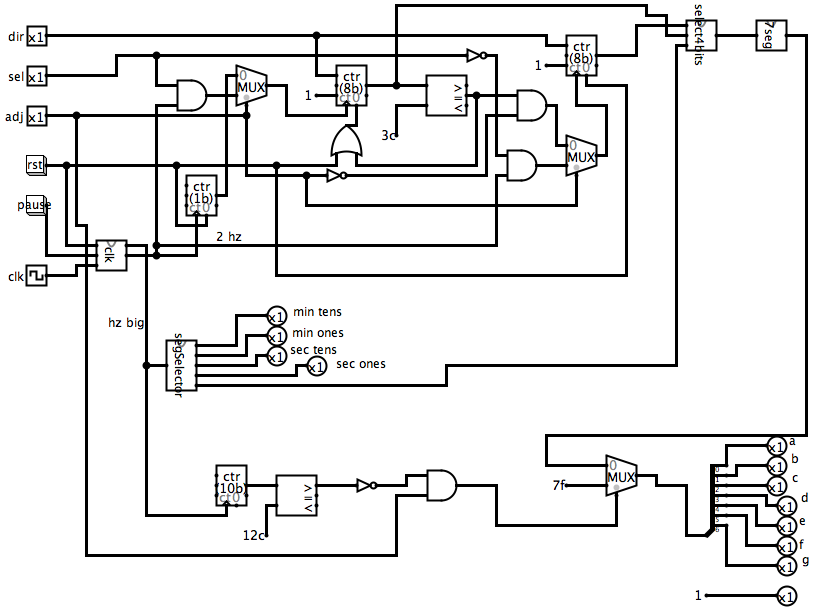
\includegraphics[width=1\textwidth]{main.png} 
		\caption{Digital Logic Design}
	\end{center}
\end{figure}

The above figure depicts the overall logic design of our circuit. The outputs a-g and p represent the segments to be lit up on the 7-segment display. The output min tens, min ones, sec tens, and sec ones represent which of the four screens on the 7-segment display should be activated where 0 corresponds with being lit up. In this figure, I black-boxed 4 components: clk, segSelector, select4bits, and 7seg. Diagrams for these components are shown below. This module uses two counters to count the minutes and seconds. The minutes are triggered by the seconds reaching 60, at which point the seconds counter overflows back to 0. Another counter is used to simulate a 1 Hz clock by controlling it with a 2 Hz clock. When reset is triggered, seconds and minutes are reset to 0, and the clock is reset back to zero as well. Pause is fed into the clock module, which will pause the 2 hz clock so that the seconds and minutes will never increment. The counter at the bottom of the screen is used to make the display blink when adjust is on. It will make the display be all 1's (all off) during a certian count, and then it will make the screen display regularly otherwise. Adjust being on will also make the seconds or minutes (depending on the select bit) increment with the 2 Hz clock. This is implemented by feeding the 1 Hz and 2 Hz clock into multiplexers, with adjust as the select bit. The output of these multiplexers goes to the clock of the counter.

\begin{figure}[H]
	\begin{center}
		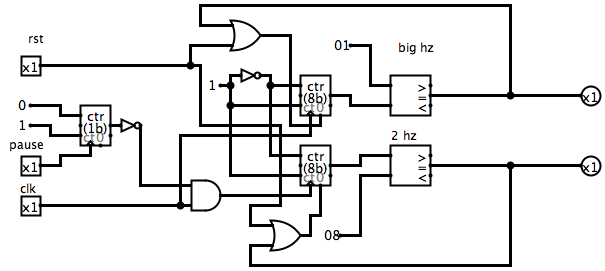
\includegraphics[width=1\textwidth]{clk.png} 
		\caption{Clock module logic}
	\end{center}
\end{figure}

This clock module takes in reset, pause, and the 100 MHz clock as input and uses counters to output a 2 Hz clock and another clock that is much faster. The counter resets after it counts to its desired Hz. A comparator is used to tell when the counter has reached a certian number. When reset is triggered, the counter will be reset to zero, and when pause is triggered, the counter will not increase.

\begin{figure}[H]
	\begin{center}
		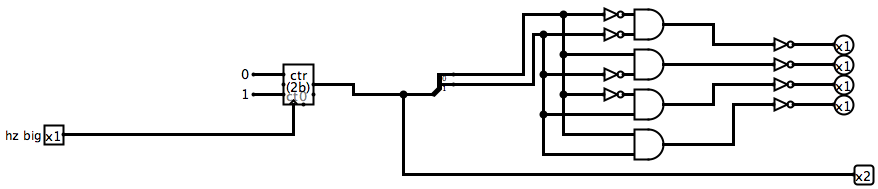
\includegraphics[width=1\textwidth]{segSelector.png} 
		\caption{Segment selector logic}
	\end{center}
\end{figure}

This module selects which of the four screens should display a digit on the seven segment display. It takes in the faster clock as an input. The output includes four bits, each bit corresponding to a screen where a 0 signifies that the screen should be lit up. The module also outputs a 2 bit integer which represents the screen number (0-3) that is being lit up this clock cycle. This module uses a counter that counts 0-3 and resets to 0 when it gets to 3 to determine which screen to light up.

\begin{figure}[H]
	\begin{center}
		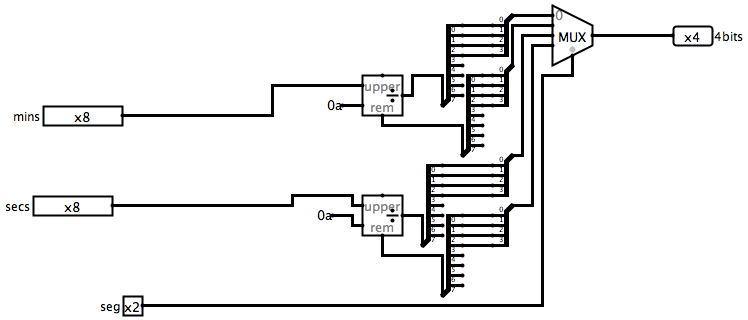
\includegraphics[width=1\textwidth]{select4bits.png} 
		\caption{Integer to display logic}
	\end{center}
\end{figure}

This module takes in as input two 8 bit integers representing the number of seconds and the number of minutes. These are fed into a divider, which essentially gets the ones and tens digits of these numbers. So we feed in the ones and tens digits of the seconds and minutes into the multiplexer, with the two bit screen integer from the segment selector module as the selector. The output is not a 4 bit integer which represents a number 0-9 to be represented on the 7 segment display. 

\begin{figure}[H]
	\begin{center}
		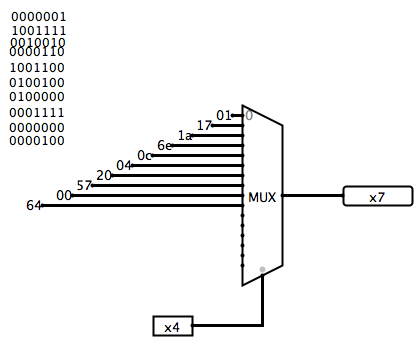
\includegraphics[width=1\textwidth]{7seg.png} 
		\caption{Four bit integer to 7 segment logic}
	\end{center}
\end{figure}

This module takes in a 4 bit integer and outputs the corresponding 7 segment display bits. The 4 bit integer is used as a selector and the left side of the multiplexer takes in 10 constants. These constants correspond to the 10 bit streams on the top of the circuit diagram. The rest are don't cares because the multiplexor should not ever get a selector that is not in the range of 0-9.

%----------------------------------------------------------------------------------------
%	SECTION 3
%----------------------------------------------------------------------------------------

\section*{Simulation}

%Simulation documentation (10%). Document all the simulation efforts (what
%requirements are tested and what the test cases are), document bugs found
%during simulation, and provide simulation waveforms. Include all simulation
%testbench code source files.
Unlike previous labs, we did not implement a test bench simulation file.  Initially, we attempted to create one for our various modules, but after having issues with uninitialized values, we chose to simply move on from this and test it via the actual FPGA board.  As to why the test bench file failed, we suspect it had to do with the clk input.  Regardless of the issue, we tested our stopwatch modules through the board using the synthesize and compilation process similar to Lab 1 (more specifically the: Synthesize->Translate->Map->Generate-> iMPACT).  
	In order to simulate our modules this way, we grabbed and modified the .ucf file from Lab 1, which allowed us to map the inputs and outputs to the correct buttons, lights, and switches on the board.  Once our code was syntactically correct, we generated a .bit file in order to implement and run the program we wrote on the board. 
	The process was generally very straightforward and smooth.  Our initial simulation effort was to light up the seven segment display; this helped us understand which values mapped to which lights allowing us to write a priority encoder of the different numbers to display.  Once that was working, we implemented clocks had to find the right speed with our fastest clock to emulate all of the 4-digits displaying at the same time without any blinking. After we had the clocks clearly working (with regards to actual, real time), we actually sped them up for testing purposes, so instead of waiting a minute to see if our minutes were decrementing correctly, we only had to wait about 30 seconds. 
	With the general clocks working, our next simulations were all based off of the various switches.  The process was relatively the same for ADJ, SEL, DIR.  ADJ worked well initially, but it had two bugs: there was no blinking of the display, which we simply forgot to code, and adjusting the seconds would eventually lead to the minutes changing as well (as in if ADJ was increasing seconds, once it hit 59, it would increment minutes by 1) .  These were both easy cases to fix, and once ADJ was working, SEL worked perfectly without any bugs to be found.  Similarly, DIR worked without any bugs on our first implementation.  We later had to test these together with the buttons, to make sure none of them lost functionality.
	After the switches were all working, we began testing the buttons.  We mapped the reset button to the center top button, and on testing it, it worked without any problems.  However, the Pause Button caused the most issues with simulation.  The debouncer was fidgety causing the pause to be inconsistent.  We tested multiple values for our debouncer, which was easily the most tedious portion of simulation, as reimplementing/compiling took nearly 4-5 minutes each time we adjusted these values.  Finally, after finding a value that we found consistent, we pressed the pause button over 300 times with a ~96\% success rate.  
	Overall, the simulation process was relatively easily, but a bit tedious.  Having to wait 4-5 minutes as well as trying to check all of the various cases to make sure things worked together was very time consuming, not to mention all of the different potential combinations was troublesome to even consider.  However, these cases, including: pausing and unpausing to make sure it stopped in between the second, reset not causing arbitrary delays, and using the different buttons with various switch combinations, all worked as the assignment specified.  


\section*{Conclusion}


%Conclusion (5%). Summary of the design. Difficulties you encountered, and
%how you dealt with them. General suggestions for improving the lab, if any.

Overall, our stopwatch design worked well, but the code itself was rather messy.  This could have been averted had we used more modules, but by the time things started getting more intricate, it wouldn't have made sense to go back and clean up what was already working.  The actual difficulties we encountered were almost all due to the debouncer for the pause button as well as the time it took to simply implement our program on the FPGA board.  Regarding the pause button: sometimes, it would be incredibly accurate, only to become less accurate the next day.  Part of this may have been which board we used (as the board the TA provided worked far more consistently), but overall, with consistent, solid presses, the pause button worked well.  
	Realistically, the only way to deal with the problem of long compilation times was by being patient.  Early on when there were still several things to implement, we would synthesize and compile, and while this was going on, we would start writing code for the next stopwatch feature.  All in all, this lab doesn't need much adjustment, however, being clearer on the various corner cases in the spec would have been helpful. 

%----------------------------------------------------------------------------------------
%	BIBLIOGRAPHY
%----------------------------------------------------------------------------------------

%\bibliographystyle{apalike}

%\bibliography{sample}

%----------------------------------------------------------------------------------------


\end{document}